%%%%%%%%%%%%%%%%%%%%%%%%%%%%%%%%%%%%%%%%%%%%%%%%%%%%%%%%%%%%%%%%%%%%%%%%%%%%%%%%%%%%%%%%%%%%%%%%%%%%%%%
%%														%%
%% 				DIPLOMOVÁ PRÁCE - Tomáš Klemsa			%%
%% 				 										%%
%%														%%
%% pro formátování využita šablona: http://geo3.fsv.cvut.cz/kurzy/mod/resource/view.php?id=775 	%%
%%													%%
%%%%%%%%%%%%%%%%%%%%%%%%%%%%%%%%%%%%%%%%%%%%%%%%%%%%%%%%%%%%%%%%%%%%%%%%%%%%%%%%%%%%%%%%%%%%%%%%%%%%%%% 

\documentclass[%
  12pt,         			% Velikost základního písma je 12 bodů
  a4paper,      			% Formát papíru je A4
  oneside,       			% Oboustranný tisk
  pdftex,				    % překlad bude proveden programem 'pdftex' do PDF
%%%  draft
]{report}       			% Dokument třídy 'zpráva'
%

\newcommand{\Fbox}[1]{\fbox{\strut#1}}

\usepackage[czech, english]{babel}	% použití češtiny, angličtiny
\usepackage[utf8]{inputenc}		% Kódování zdrojových souborů je UTF8

\usepackage[square,sort,comma,numbers]{natbib}

\usepackage{caption}
\usepackage{subcaption}
\captionsetup{font=small}
\usepackage{enumitem} 
\setlist{leftmargin=*} % bez odsazení

\makeatletter
\setlength{\@fptop}{0pt}
\setlength{\@fpbot}{0pt plus 1fil}
\makeatletter

\usepackage[dvips]{graphicx}   
\usepackage{color}
\usepackage{transparent}
\usepackage{wrapfig}
\usepackage{float} 

\usepackage{cmap}           
\usepackage[T1]{fontenc}    

\usepackage{textcomp}
\usepackage[compact]{titlesec}
\usepackage{amsmath}
\addtolength{\jot}{1em} 

\usepackage{chngcntr}
\counterwithout{footnote}{chapter}

\usepackage{acronym}

\usepackage[
    unicode,                
    breaklinks=true,        
    hypertexnames=false,
    colorlinks=true, % true for print version
    citecolor=black,
    filecolor=black,
    linkcolor=black,
    urlcolor=black
]{hyperref}         

\usepackage{url}
\usepackage{fancyhdr}
%\usepackage{algorithmic}
\usepackage{algorithm}
\usepackage{algcompatible}
\renewcommand{\ALG@name}{Pseudokód}% Update algorithm name
\def\ALG@name{Pseudokód}

\usepackage[
  cvutstyle,          
  diploma        
]{thesiscvut}


\newif\ifweb
\ifx\ifHtml\undefined % Mimo HTML.
    \webfalse
\else % V HTML.
    \webtrue
\fi 

\renewcommand{\figurename}{Obrázek}
\def\figurename{Obrázek}

%%%%%%%%%%%%%%%%%%%%%%%%%%%%%%%%%%%%%%%%%%%%%%%%%%%%%%%%%%%%%%%%%
%%%%%%%%%%% Definice informací o dokumentu  %%%%%%%%%%%%%%%%%%%%%
%%%%%%%%%%%%%%%%%%%%%%%%%%%%%%%%%%%%%%%%%%%%%%%%%%%%%%%%%%%%%%%%%

%% Název práce
\nazev{Název}
{Title}

%% Jméno a příjmení autora
\autor{Tomáš}{Klemsa}

%% Jméno a příjmení vedoucího práce včetně titulů
\garant{Jméno vedoucího}

%% Označení oboru studia
\oborstudia{Geomatika}{}

%% Označení ústavu
\ustav{Katedra geomatiky}{}

%% Rok obhajoby
\rok{2020}

%Mesic obhajoby
\mesic{červen}

%% Místo obhajoby
\misto{Praha}

%% Abstrakt
\abstrakt 
{ 	\parindent=1cm Abstrakt....................................... }
{	\parindent=1cm Abstract.......................................  }

%% Klíčová slova
\klicovaslova
{klíčová slova}
{Key worlds}

%%%%%%%%%%%%%%%%%%%%%%%%%%%%%%%%%%%%%%%%%%%%%%%%%%%%%%%%%%%%%%%%%%%%%%%%

%%%%%%%%%%%%%%%%%%%%%%%%%%%%%%%%%%%%%%%%%%%%%%%%%%%%%%%%%%%%%%%%%%%%%%%%
%% Nastavení polí ve Vlastnostech dokumentu PDF
%%%%%%%%%%%%%%%%%%%%%%%%%%%%%%%%%%%%%%%%%%%%%%%%%%%%%%%%%%%%%%%%%%%%%%%%
\nastavenipdf
%%%%%%%%%%%%%%%%%%%%%%%%%%%%%%%%%%%%%%%%%%%%%%%%%%%%%%%%%%%%%%%%%%%%%%%

%%% Začátek dokumentu
\begin{document}

\catcode`\-=12  % pro vypnuti aktivniho znaku '-' pouzivaneho napr. v \cline 

% aktivace záhlaví
\zahlavi

% předefinování vzhledu záhlaví
\renewcommand{\chaptermark}[1]{%
	\markboth{\MakeUppercase
	{%
	\thechapter.%
	\ #1}}{}}

% Vysázení přebalu práce
%\vytvorobalku

% Vysázení titulní stránky práce
\vytvortitulku

% Vysázení listu zadani
\stranka{}%
	%{\includegraphics[scale=0.7]{./zadani.jpg}}%\sffamily\Huge\centering\ }%ZDE VLOŽIT LIST ZADÁNÍ}%
	%{\sffamily\centering Z~důvodu správného číslování stránek}

% Vysázení stránky s abstraktem
\vytvorabstrakt

% Vysázení prohlaseni o samostatnosti
\vytvorprohlaseni

% Vysázení poděkování
\stranka{%nahore
       }{%uprostred
       }{%dole
       \sffamily
	\begin{flushleft}
		\large
		\MakeUppercase{Poděkování}
	\end{flushleft}
	\vspace{1em}
		%\noindent
	\par\hspace{2ex}
	{Poděkování...}
}


% Vysázení obsahu
\obsah

% Vysázení seznamu tabulek
%\seznamtabulek

% jednotlivé kapitoly
\chapter{Úvod}
	Fotogrammetrie je obor zabývající se geometrickými vztahy mezi objekty zachycenými na fotografickém snímku. Tento způsob se často využívá u dokumentace historických objektů, tvorby map z leteckých snímků, při dokumentaci dopravních nehod atd. Fotogrammetrii můžeme rozdělit do více kategorií.
	
	\textbf{Jednosnímková fotogrammetrie}
	
	Nejjednodušší metoda je tzv. jednosnímková fotogrammetrie. Jak název napovídá, je zpracováván pouze jeden snímek. Metoda je hojně využívána u dokumentace fasád budov. Omezení při tomto postupu je, že ze snímku získáme pouze dvojrozměrnou informaci, proto jakákoliv hloubková členění budou oproti zvolené rovině zkreslená.
	
	\textbf{Stereofotogrammetrie}
	
	Metoda využívající stereoskopického vjemu, na jehož základě získáme z dvou překrývajících se snímků s rovnoběžnou osou záběru prostorové informace. Tato metoda je hojně využívána v letecké fotogrammetrii.

	\textbf{Průseková fotogrammetrie}
	
	Průseková fotogrammetrie využívá více snímků s nerovnoběžnou osou záběru, na kterých jsou vyhledány identické body, ze kterých jsou získané prostorové souřadnice těchto bodů.
	
	\textbf{Obrazová korelace}
	
	
	Obrazová korelace, hojně nazývána také jako IBMR (\textit{Image Based Modeling and Rendering}) je metoda využívající obrazovou korelaci pro vyhledávání identických bodů. Funguje v podstatě na principu průsekové fotogrammetrie s tím rozdílem, že je potřeba velké množství snímků a algoritmus SIFT (\textit{Scale Invariant Feature Transformation}), který vyhledává identické body, proto je vhodná pro objekty negeometrického tvaru.
	
	Všechny tyto metody využívají obrazová data, u kterých je předpoklad středového promítání. To ovšem u fotoaparátů s běžným objektivem neplatí. Fotografie jsou zatíženy geometrickým zkreslením, které by se projevilo na kvalitě výstupu. Proto je nutné toto zkreslení redukovat.

	Tato bakalářská práce je zaměřena na tvorbu jednoduchého a uživatelsky přívětivého softwaru pro odstranění geometrického zkreslení fotografických snímků na základě znalosti prvků vnitřní orientace včetně průběhu radiální a tangenciální distorze. Průběh distorze může být vyjádřen různými způsoby. Pro tvořený program byl však zvolen model podle Duane C. Browna, který je často využívaným modelem ve fotogrammetrických softwarech.
	
	Existuje mnoho programů, které umí nežádoucí zkreslení ze snímků odstranit. Proč tedy vyvíjet nástroj nový? 
	
	Jako první bych zmínil grafické editory. Jedná se o nástroje, které většinou umí odstranit zkreslení na základě subjektivního vnímání uživatele. Například tak, že posuvníkem uživatel nastavuje velikost zkreslení, až stěny budovy nejsou prohnuté. Tyto nástroje jsou ovšem vhodné pouze pro fotografie, které nebudou fotogrammetricky zpracovávány. Nepracují totiž s tangenciální distorzí, souřadnicemi hlavního snímkového bodu a nastavení průběhu radiální distorze je často velmi omezené. 
	
	Do druhé skupiny bych zařadil programy fotogrammetrické. Často profesionální a velmi obsáhlý software, který je ovšem v mnohých případech finančně nákladný. V některých případech tyto programy mají funkci na poloautomatický výpočet prvků vnitřní orientace, což je značná úspora času.\par


\section{Cíle práce}
	Cílem této práce je tedy vytvořit program, který bude volně šiřitelný, aby kdokoliv měl možnost upravovat, šířit a dále využívat zdrojový kód a bude psán v rozšířeném multiplatformním objektově orientovaném programovacím jazyce, tak aby byla snadná jeho další úprava. Program byl tedy vytvořen v jazyce \textit{C++} na platformě \textit{Qt}.


\chapter{Rešerše používaných algoritmů}
Tato kapitola se zabývá přehledem používaných algoritmů pro výpočet polygonů ze vstupních linií. Polygonizace, v případě výskytu fuzzy průsečíků, se zpravidla neřeší jedním algoritmem na polygonizaci, ovšem průsečíky linií jsou nejprve doplněny a poté se zahájí vlastní tvorba polygonů z těchto upravených linií. Toto řešení používají i v praxi užívané GIS nástroje, jako například nástroj \textit{"Polygonize"} využívaný v softwaru \textit{QGis}, nebo nástroj \textit{"Feature To Polygon"} ze softwaru \textit{ArcGIS}.

\textbf{TODO: tady by bylo fajn citovat buďto dokumentaci QGis nebo vlastní repozitář... u arcgis je toto tvrzení založeno jen na výstupu aplikace v task history.}

\section{Výpočet průsečíků množiny linií}
Výpočet všech průsečíků množin linií lze provést snadno, testováním všech úseček se všemi. Tímto postupem ovšem zjevně dosáhneme složitosti $\mathcal{O}(N^2)$. Pro výpočet průsečíků lze ovšem využít i algoritmus s časovou náročnosti $\mathcal{O}(n\log{}n)$, známý také jako Bentley–Ottmannův algoritmus \cite{bentley1979algorithms}.

\subsection{Vzájemná poloha dvou úseček}
Ve 2D výpočetní geometrii jsou standardně jednotlivé segmenty linie vyjádřeny počátečním a koncovým bodem. Uvažujme tedy že máme dány 2 přímky $p_1 = |S_1 E_1|$ a $p_2 = |S_2 E_2|$, kde $S_1 = [x_{S1},y_{S1}]$, $E_1 = [x_{E1},y_{E1}]$, $S_2 = [x_{S2},y_{S2}]$, $E_2 = [x_{E2},y_{E2}]$ a potřebujeme provést test, zda se dané přímky protínají či nikoliv, můžeme použít takzvaný \textit{Half-Plane} test, tedy test, který určuje zda bod leží v pravé či levé polorovině od přímky. Tento test zopakujeme celkem čtyřikrát a to na počáteční a koncový bod druhé úsečky, abysme zjistili zda se přímky protínají. Test je založen na výpočtu orientace dvou vektorů $\vec{u}$  a $\vec{v}$, kde vektor $\vec{v}$ je směrový vektor úsečky, tedy $\overrightarrow{S_1E_1}$ a vektor $\vec{v}$ je vektor $\overrightarrow{S_1S_2}$.

	

	

\begin{figure}[h]
  \centering
  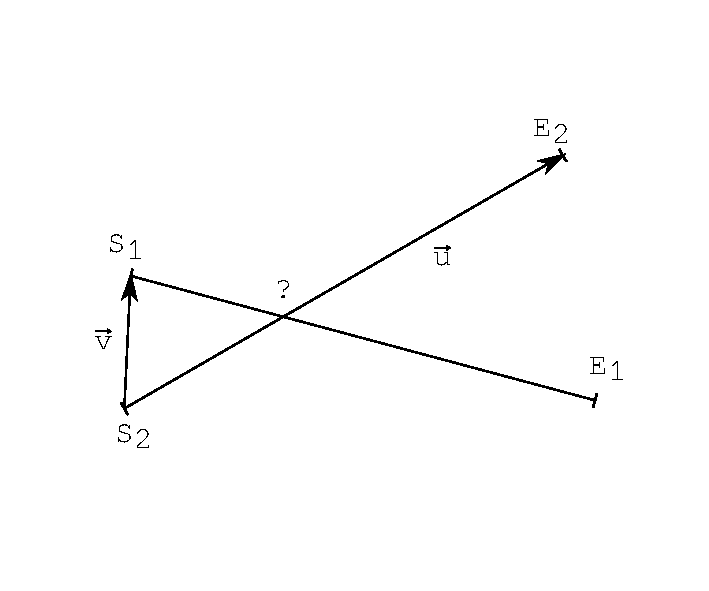
\includegraphics[width=12cm]{./pictures/2/half-plane_vector.pdf}
  \caption{\textit{Half-plane} test}
  \label{fig:2-half_plane_vector}
\end{figure}

\begin{figure}[h]
    \centering % <-- added
\begin{subfigure}{0.5\textwidth}
  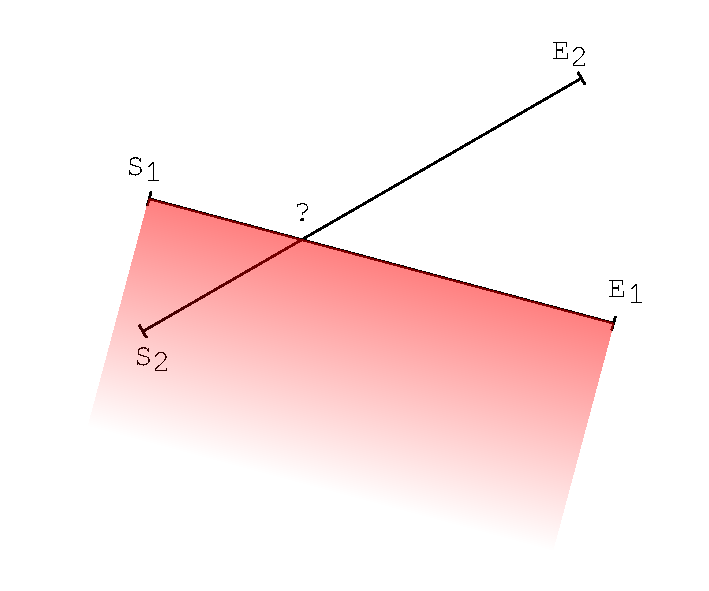
\includegraphics[width=\linewidth]{./pictures/2/half-plane_1.pdf}
  \caption{Test bodu $S_2$ k přímce $|S_1E_1|$}
  \label{fig:2-half_plane_1}
\end{subfigure}\hfil % <-- added
\begin{subfigure}{0.5\textwidth}
  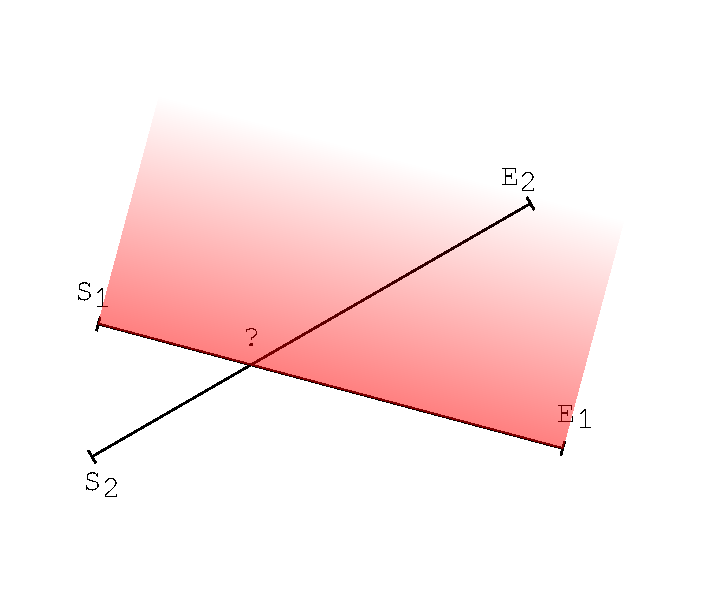
\includegraphics[width=\linewidth]{./pictures/2/half-plane_2.pdf}
  \caption{Test bodu $E_2$ k přímce $|S_1E_1|$}
  \label{fig:2-half_plane_2}
\end{subfigure}\hfil % <-- added

\medskip
\begin{subfigure}{0.5\textwidth}
  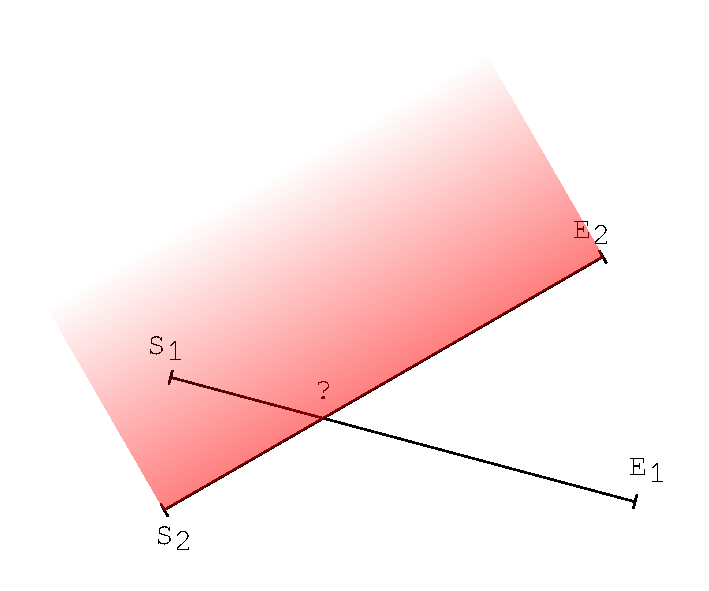
\includegraphics[width=\linewidth]{./pictures/2/half-plane_3.pdf}
  \caption{Test bodu $S_1$ k přímce $|S_2E_2|$}
  \label{fig:2-half_plane_3}
\end{subfigure}\hfil % <-- added
\begin{subfigure}{0.5\textwidth}
  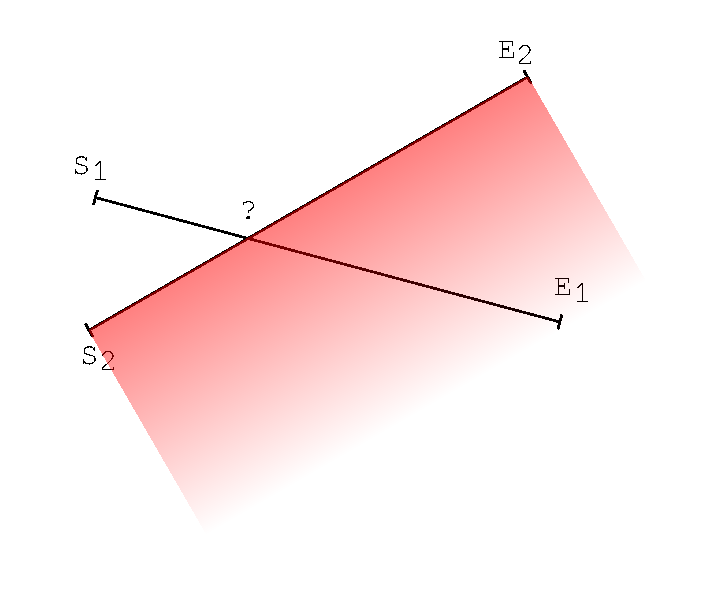
\includegraphics[width=\linewidth]{./pictures/2/half-plane_4.pdf}
  \caption{Test bodu $E_1$ k přímce $|S_2E_2|$}
  \label{fig:2-half_plane_4}
\end{subfigure}\hfil % <-- added
\caption{Grafické znázornění \textit{Half-plane} testů pro zjištění existence průsečíku}
\label{fig:2-half_plane}
\end{figure}

\subsection{Bentley–Ottmannův algoritmus}
Tento algoritmus je založen na technice zvané \textit{sweep line}, překládané jako \textit{zametací přímka}, pro kterou je předpokladem mít setříděná vstupní data, podle jedné ze souřadnic. Algoritmus zde nebuda více popisován jelikož je velmi dobře vysvětlen v těchto publikacích \cite{bentley1979algorithms} \cite{bayer2008algoritmy}.

\section{Polygonizace}
Jak již bylo řečeno, polygonizace se provádí nad daty s doplněnými průsečíky linií. Doplnění průsečíku jsme schopni vyřešit v čase $\mathcal{O}(n\log{}n)$. Nyní tedy nastává otázka jak řešit vlastní polygonizaci.


\section{GIS software}
Provedení polygonizace zvládá většina současně používaného GIS softwaru. Pokusíme se tedy rozebrat postupy jednotlivých nástrojů na polygonizaci.

\subsection{ArcGIS}
ArcGIS je vyvíjený společností Esri, v současné době se jedná o nejpokročilejší nástroj v oblasti GIS. Jedná se o proprietární software, u kterého 


\subsection{QGis}
QGis je nejspíše jeden z nejznámějších volných nástrojů pro práci v GIS. Je šířen pod copyleftovou  licencí \textit{GNU General Public License}, tudíž máme volný přístup ke zdrojovému kódu aplikace dostupných v online repozitářích. To nám umožňuje nahlížet do výpočetních algoritmů, které jsou v případě QGis psány v programovacím jazyce \textit{C++} a \textit{Python}, narozdíl od komerčních nástrojů, které si implementaci často chrání

\subsection{Grass GIS}

\subsection{PostGis}

\chapter{Závěr}
\label{9-zaver}

		V této práci byla zpracována stručná rešerše literatury, zabývající se metodami odstranění zkreslení z fotografických snímků. Vybrané metody odstranění zkreslení jsou dále v práci popsány. Jako nejvhodnější způsob se jevilo odstranění zkreslení za pomoci \textit{Brownova} distorzního modelu, který je v obdobných softwarech často používaný.
	
	Hlavním cílem této práce bylo vytvořit softwarové řešení tohoto problému, které bude mít moderní grafické rozhraní. Pro tvorbu softwaru byl zvolen programovací jazyk \textit{C++} s využitím knihoven \textit{Qt}. Tento nástroj usnadnil tvorbu grafického rozhraní, které je zkoncipováno tak, aby mohl uživatel intuitivně program ovládat a nebylo zapotřebí podrobnější znalosti softwaru. Program byl sestaven pro platformu \textit{Windows}, jelikož je však jazyk \textit{C++} s knihovnami \textit{Qt} určen pro různé platformy, nic nebrání tento program sestavit i pro \textit{Linux} či \textit{macOS}, což tento software dělá použitelnější pro větší okruh lidí. Dalším vylepšením vytvořeného programu \textit{DistortionRemover} by do budoucna mohlo být obohacení o výpočet parametrů prvků vnitřní orientace kamery, které v současné době musí uživatel získat z jiného softwaru, či jiného zdroje. Velkým zlepšením by mohlo také být práce s obrazovými daty typu RAW, zamezilo by se tak velkým ztrátám kvality při opravě snímku. Samozřejmostí je opravení chyb, v programu, které budou odhaleny rozsáhlejším používáním. 
		
	Ve finální části, je předvedena práce s programem na příkladu historického stavebního objektu z databáze PhotoPa a jsou nastíněny další možné postupy zpracování.

	




% Vysázení seznamu zkratek
%
\begin{seznamzkratek}{ABCDE}

	\novazkratka{GIS}
	      {GIS}
	      {Geografický informační systém}

      \novazkratka{OSGeo}
	      {OSGeo}
	      {Open Source Geospatial Foundation}
      
      \novazkratka{GEOS}
	      {GEOS}
	      {Geometry Engine, Open Source}
	      
	  \novazkratka{OGC}
	      {OGC}
	      {Open Geospatial Consortium}
	      
	      
	      
	  \novazkratka{GPL}	
	      {GPL}
	      {Všeobecná veřejná licence (General Public License)}
	      
	  \novazkratka{LGPL}	
	      {LGPL}
	      {Lesser General Public License}
	      
	   \novazkratka{SPI}	
	      {SPI}
	      {Java Service Provider Interface}
	      
	   \novazkratka{JDBC}	
	      {JDBC}
	      {Java Database Connectivity}
	      
	   \novazkratka{API}	
	      {API}
	      {Aplication Interface}
	      
	   \novazkratka{RGB}	
	      {RGB}
	      {Barevný model Red, Green, Blue}

	   \novazkratka{GDF/DIME}	
	      {GDF/DIME}
	      {Geographic Base File/Dual Independent Map Encoding}
	      
	      

\end{seznamzkratek}

% Vysázení seznamu obrázků
\seznamobrazku/obrazky

% Literatura
\nocite{*}
\def\refname{Literatura}
\bibliographystyle{mystyle}
\bibliography{literatura}

%% Začátek příloh
\def\figurename{Figure}%
\prilohy
%
%% Vysázení seznamu příloh
%\seznampriloh
%
%% Vložení souboru s přílohami
%%%%%%%%%%%%%%%%%%%%%%%%%%%%%%%%%%%%%%%%%%%%%%%%%%%%%%%%%%%%%%%%%%%%%%%%%%%%%%%%%%%
%%                 PŘÍLOHA - UŽIVATELSKÁ PŘÍRUČKA                                %%
%%%%%%%%%%%%%%%%%%%%%%%%%%%%%%%%%%%%%%%%%%%%%%%%%%%%%%%%%%%%%%%%%%%%%%%%%%%%%%%%%%%
\chapter{Srovnání polygonizace v ArcGIS Desktop a QGIS Desktop}
\label{chap:srovnani}
Srovnání bylo provedeno na testovacích datech, které poskytl \textit{Ing. Jan Růžička, Ph.D.}. Jelikož nemohla být poskytnuta reálná data, jedná se o uměle vygenerované linie, které jsou dle slov doktora Růžičky obdobného charakteru a velikosti. Data obsahují celkem 10000 linií. Tato data byla dále testována ve zmenšené formě a to s 1000 a 100 liniemi.

\section{Parametry počítače}
\begin{itemize}
\item \textbf{Operační systém:} 
\item \textbf{Procesor:} 
\item \textbf{RAM:} 
\end{itemize}

\section{ArcGIS Desktop}

\section{QGIS Desktop}


\chapter{Elektornické přílohy}
\label{user-guide}

\section{CD disk}

\pagenumbering{Roman}
\label{app:cd}
    
    \begin{description}
        \item[\tt BP-DistortionRemover.pdf] ~ \\ text bakalářské práce ve formátu *.pdf,
    	
        
        \item[\tt DistortionRemover/] ~ \\ adresář s programem,
        \begin{description}
        		
        		\item[\tt DistortionRemover.exe] ~ \\ Spustitelný soubor aplikace,
        		
        		\item[\tt License.txt] ~ \\ textový soubor s popisem licence,
        		
            	\item[\tt Source/] ~ \\ adresář obsahující zdrojové kódy,
            	\begin{description}
            			\item[\tt DistortionRemover.pro] ~ \\ projektový soubor,
            			\item[\tt main.cpp] ~ \\ zdrojový kód funkce main,
            			\item[\tt distortionremover.h] ~ \\ hlavičkový soubor distortionremover,
            			\item[\tt distortionremover.cpp] ~ \\ zdrojový soubor distortionremover obsahující funkce pro chod programu,
            			\item[\tt ui\_distortionremover.h] ~ \\ hlavičkový soubor grafického rozhraní,
            			\item[\tt distortionremover.ui] ~ \\ soubor obsahující grafické prostředí v XML,
            			\item[\tt picturetransformation.h] ~ \\ hlavičkový soubor picturetransformation,
            			\item[\tt picturetransformation.cpp] ~ \\ zdrojový soubor picturetransformation obsahující výpočetní funkce,
            			\item[\tt resource.qrc] ~ \\ soubor pro uložení binárních souborů do aplikace který obsahuje ikonu,
            			\item[\tt DR.ico] ~ \\ ikona programu.

            	\end{description}
        \end{description}
    \end{description}



% Konec dokumentu
\end{document}

